\documentclass[a4paper, 12pt]{article}

\usepackage[ a4paper,
 total={170mm,257mm},
 left=20mm,
 top=20mm,]{geometry}

\usepackage{cmap}
\usepackage[T2A]{fontenc}
\usepackage[utf8]{inputenc}
\usepackage[english, russian]{babel}

%Графика
\usepackage{graphicx}
\usepackage{float}%"Плавающие" картинки
\usepackage{wrapfig}%Обтекание фигур (таблиц, картинок и прочего)
\graphicspath{{./images/}}

% Математика
\usepackage{amsmath,amsfonts,amssymb,amsthm,mathtools} 

%Title Page
\title{ЛАБОРАТОРНАЯ РАБОТА № 3 \\
Моделирование различных форм резервуаров с жидкостью
}
\author{Вариант 11 \\ Машуров Владимир БПМ-19-3}

\setcounter{page}{0}

\begin{document}
\maketitle
\thispagestyle{empty}
\newpage
\tableofcontents

\section{Простой цилиндрический резервуар с жидкостью}

Обратим внимание на рисунок \ref{p:Простой_цилиндрический_резервуар}, там приведёт пример рассматриваемого резервуара с жидкостью или пульпой. \\
$V$ – объём жидкости; \\
$S$ – площадь поверхности жидкости; \\
$Q_1,\ Q_2$  – объёмные расходы жидкости; \\ 
$F$ – площадь проходного отверстия сливной трубы. Расход $Q_2$ \\ принимается в качестве управляющего воздействия. \\


\begin{figure}[h!]
	\centering
	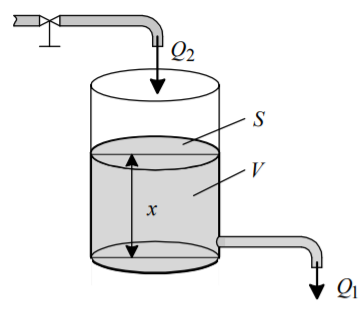
\includegraphics[scale=0.8]{example_1}
	\caption{Простой цилиндрический резервуар с жидкостью  }
	\label{p:Простой_цилиндрический_резервуар}
\end{figure}

Запишем уравнение материального баланса жидкости для данного резервуара:
$$ \Delta V + Q_1 * \Delta t = Q_2 \Delta t $$ 

Предположим, что $\Delta t \to 0$ и $\Delta V \to 0$, тогда разделим на $\Delta t$ и получим:
$$\dot{V}+Q_1=Q_2; $$

Объём жидкости V выражается через её уровень x: $V = S \cdot x $. Найдем изменение объема жидкости: $\dot{V}=S\ast\dot{x} $. Далее, зависимость между объёмным расходом $Q_1$ и уровнем x вытекает из
уравнения Д. Бернулли (Bernoulli), получим: 
$$\frac{\rho\cdot v_0^2}{2}+\ \rho\cdot\ g\cdot\ x+P_1=\ \frac{\rho\cdot v^2}{2} + \rho\cdot\ g\cdot\ x_0+p_2$$

где $v$ -- скорость истечения жидкости из сливного отверстия; $v_0$ -- скорость изменения уровня жидкости в резервуаре; $x_0 - x$ -- перепад высот жидкости в резервуаре; $p1, p2$ -- статические давления над жидкостью в резервуаре и за сливным отверстием; $\rho$ -- плотность жидкости; $g$ -- ускорение свободного падения. Величина $\frac{\rho v^2}{2}$ называется динамическим или скоростным давлением. Это уравнение можно переписать в виде

$$\frac{v^2-v_0^2}{2 \cdot g}=\ \frac{p_1-p_2}{\gamma}+\left(x-x_o\right)$$
где $\gamma = \rho g$ -- удельный вес.

В предположении, что $v_0 >> v$ , $x_0 - x$ , $p_1 = p_2$ , скорость истечения жидкости будет определяться выражением $v = \sqrt{2 g x}$. При умножении левой и правой частей этого выражения на площадь проходного сечения $F$ , получается: 

$$ Fv = Q_1 = F \sqrt{2gx} $$

С помощью поправочного коэффициента $\mu$, чаще всего определяемого экспериментально, может быть учтена форма и состояние поверхности сливного отверстия. Например, для отсадочной машины рекомендуется значение $\mu = 0.6$.

$$Q_1=\mu F\sqrt{2gx}$$

Найденное выражение подставляется в ДУ изменения объёма жидкости: 

$$ S \frac{\partial x}{\partial t} + \mu F \sqrt{2gx} = Q_2 $$

При $\frac{\partial x}{\partial t} = 0$ можно записать уравнение статического (стационарного) режима резервуара:

$$ \mu F \sqrt{2gx} = Q_2$$

\begin{figure}[h!]
	\centering
	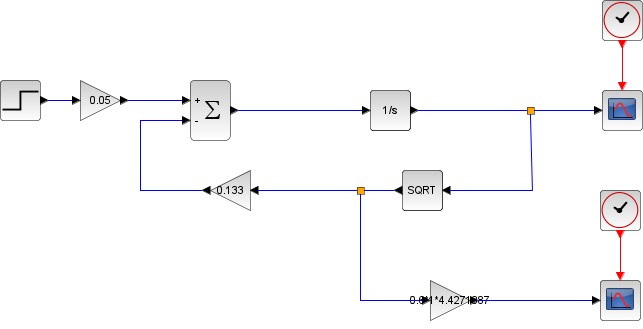
\includegraphics[scale=0.7]{scheme1}
	\caption{Структурная схема моделирования простого цилиндрического резервуара с жидкостью}
	\label{p:Простой_цилиндрический_резервуар_схема}
\end{figure}

\begin{figure}[h!]
	\centering
	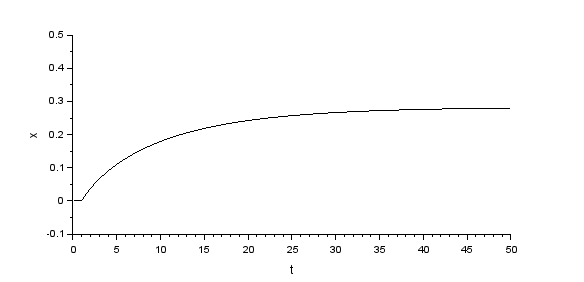
\includegraphics[scale=0.8]{graph1-1}
	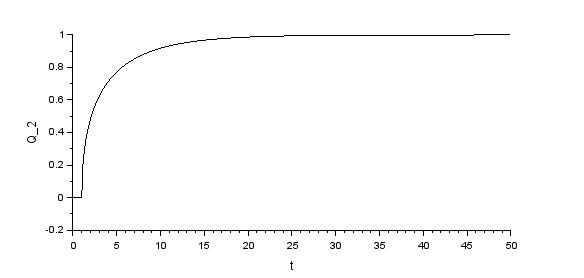
\includegraphics[scale=0.8]{graph1-2}
	\caption{Графики изменения уровня (сверху) жидкости/пульпы в простом цилиндрическом резервуаре и объема расхода жидкости (снизу), поступающей в резервуар}
	\label{p:Простой_цилиндрический_резервуар_графики}
\end{figure}

Приняв:
$S = 2 \ m^2$; 
$\mu = 0.6 $;  
$F = 1 \ m^2$;  
$g = 9.8 \ \frac{m}{s^2}$ 

На рисунке \ref{p:Простой_цилиндрический_резервуар_схема} приведена схема моделирования процессов, протекающих в простом цилиндрическом резервуаре. На рисунке \ref{p:Простой_цилиндрический_резервуар_графики} приведены графики, полученные при моделировании. 

\newpage
%-----------------------------------------------------------------

\section{Резервуар формы усеченного конуса}

\begin{figure}[h!]
	\centering
	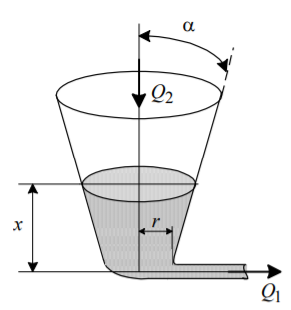
\includegraphics[scale=0.8]{example_2}
	\caption{ Резервуар формы усеченного конуса с жидкостью  }
	\label{p:Простой_резервуар_конус}
\end{figure}

Обратим внимание на рисунок \ref{p:Простой_резервуар_конус}, там приведёт пример рассматриваемого резервуара с жидкостью или пульпой. \\
$\alpha$ -- угол стенки конуса относительно основания; \\
$S$ -- площадь поверхности жидкости; \\
$Q_1,\ Q_2$  – объёмные расходы жидкости; \\ 
$r$ -- радиус окружности сечения конуса параллельной основанию; \\
$x$ -- высота уровня жидкости \\
$F$ – площадь проходного отверстия сливной трубы. Расход $Q_2$ принимается в качестве управляющего воздействия; 

Уравнение площади поверхности жидкости при достижении ею определенного уровня:
\[ S\left(x\right)=\ \pi(R^2+2\cdot\ R\cdot\tan{\alpha}+\ {(tan{\alpha})}^2\cdot\ x^2) \]

Дифференциальное уравнение процесса:
\[ \frac{dx}{dt}=\frac{Q_2}{{\pi(r}^2+2r\tg{\alpha x}+\tg^2{\alpha x^2})}-\frac{\mu F\sqrt{2gx}}{{\pi(r}^2+2r\tg{\alpha x}+\tg^2{\alpha x^2)}} \]

Приняв:
$R = 2 \ m^2$; 
$\mu = 0.6 $;  
$F = 5 \ m^2$;  
$g = 9.8 \ \frac{m}{s^2}$; 
$Q_2 = 5 \ \frac{m^3}{s}$; 
$\alpha = 45^o $

На рисунке \ref{p:конический_резервуар_схема} приведена схема моделирования процессов, протекающих в коническом резервуаре. На рисунке \ref{p:конический_резервуар_графики} приведены графики, полученные при моделировании. 

\begin{figure}[h!]
	\centering
	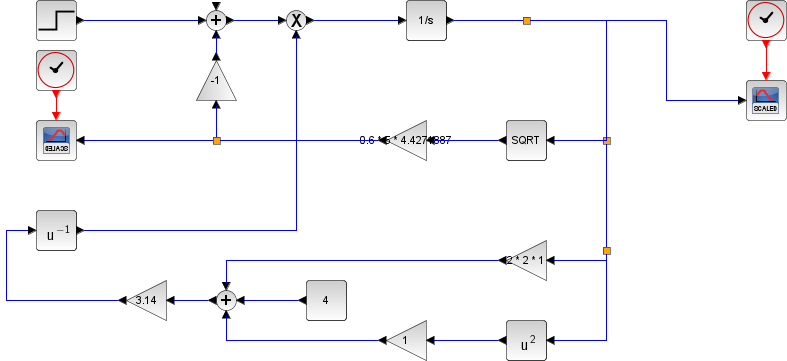
\includegraphics[scale=0.5]{scheme2}
	\caption{Структурная схема моделирования конического резервуара с жидкостью}
	\label{p:конический_резервуар_схема}
\end{figure}


\begin{figure}[h!]
	\centering
	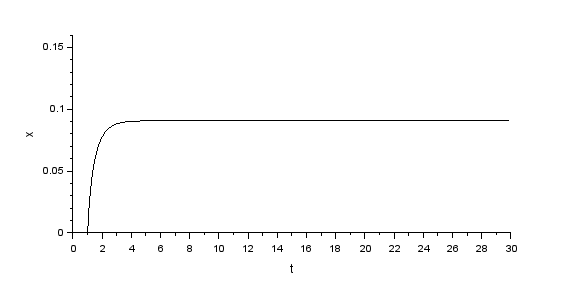
\includegraphics[scale=0.8]{graph2-2}
	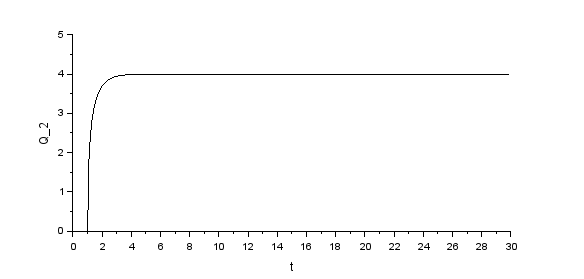
\includegraphics[scale=0.8]{graph2-1}
	\caption{Графики изменения уровня (сверху) жидкости/пульпы в коническом резервуаре и объема расхода жидкости (снизу), поступающей в резервуар}
	\label{p:конический_резервуар_графики}
\end{figure}

\newpage
%---------------------------------------------------------------

\section{Резервуар сферической формы}

\begin{figure}[h!]
	\centering
	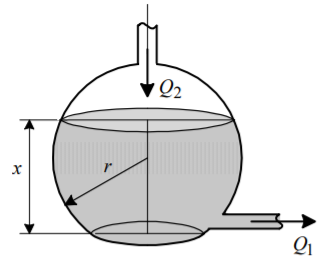
\includegraphics[scale=0.8]{example_3}
	\caption{ Резервуар сферической формы  }
	\label{p:Резервуар_сфера}
\end{figure}

Обратим внимание на рисунок \ref{p:Резервуар_сфера}, там приведёт пример рассматриваемого резервуара с жидкостью или пульпой. \\
$S$ -- площадь поверхности жидкости; \\
$Q_1,\ Q_2$  – объёмные расходы жидкости; \\ 
$r$ -- радиус сферы; \\
$x$ -- высота уровня жидкости; \\
$F$ – площадь проходного отверстия сливной трубы. Расход $Q_2$ принимается в качестве управляющего воздействия. 

Уравнение площади поверхности жидкости при достижении ею определенного уровня:
\[ S = S(x) = \pi(2\ast\ r\ast\ x-\ x^2) \]

Дифференциальное уравнение процесса:
\[ \frac{dx}{dt}=\frac{Q_2}{\pi\left(2rx-x^2\right)}-\frac{\mu F\sqrt{2gx}}{\pi\left(2rx-x^2\right)} \]

Приняв:
$R = 2 \ m^2$; 
$\mu = 0.6 $;  
$F = 1 \ m^2$;  
$g = 9.8 \ \frac{m}{s^2}$; 
$Q_2 = 5 \ \frac{m^3}{s}$; 

На рисунке \ref{p:сферический_резервуар_схема} приведена схема моделирования процессов, протекающих в сферическом резервуаре. На рисунке \ref{p:сферический_резервуар_графики} приведены графики, полученные при моделировании. 

\begin{figure}[h!]
	\centering
	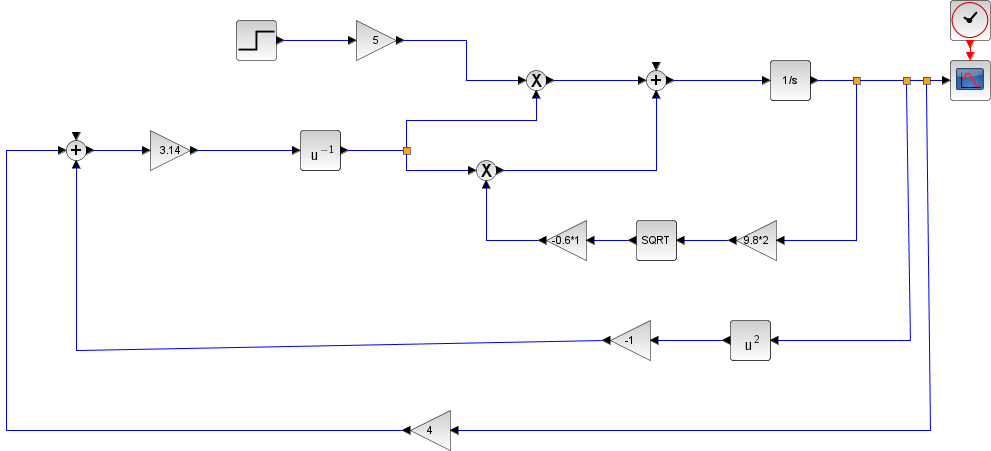
\includegraphics[scale=0.5]{scheme3}
	\caption{Структурная схема моделирования сферического резервуара с жидкостью}
	\label{p:сферический_резервуар_схема}
\end{figure}


\begin{figure}[h!]
	\centering
	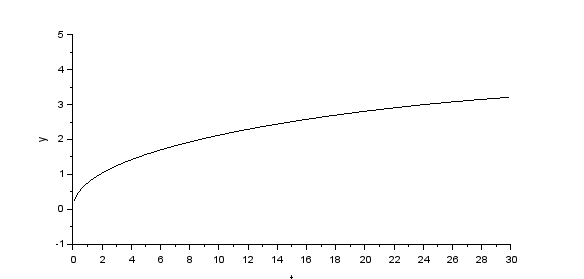
\includegraphics[scale=0.8]{graph3-1}
	\caption{Графики изменения уровня жидкости/пульпы в сферическом резервуаре }
	\label{p:сферический_резервуар_графики}
\end{figure}

\newpage
%------------------------------------------------------------

\section{Флотационная машина}
 
\begin{figure}[h!]
	\centering
	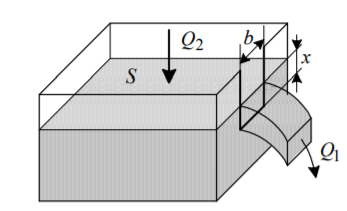
\includegraphics[scale=0.8]{example_4}
	\caption{ Флотационная машина  }
	\label{p:Флотационная_машина}
\end{figure}

Обратим внимание на рисунок \ref{p:Флотационная_машина}, там приведёт пример флотационной\footnote{ Флотация – способ обогащения полезных ископаемых, основанный на различной смачиваемости водой поверхности частиц, особенно после обработки флотационными реагентами} машины. \\

Истечение жидкости происходит в соответствии с нелинейным ДУ:
\[ S\dot{x}+\left(0.465+\frac{0.003}{x}\right)b\sqrt{2gx}\cdot x = Q_2 \]

Статическая зависимость (нагрузочная характеристика) :
\[ \frac{dx}{dt}=\frac{Q_2}{S}-\frac{0,465bx\sqrt{2gx}}{S}-\frac{0.003b\sqrt{2gx}}{S} \]

Характеризует физический закон слива жидкости через порог. Здесь зависимость расхода жидкости $Q_1$ от её уровня $x$ приводится в виде эмпирической формулы. \\
$S$ -- площадь поверхности жидкости; \\
$Q_1,\ Q_2$  – объёмные расходы жидкости; \\ 
$x$ -- высота уровня жидкости; \\
$b$ -- ширина сливного отверстия; \\
$F$ -- площадь проходного отверстия сливной трубы. Расход $Q_2$ принимается в качестве управляющего воздействия;

Приняв:
$S = 50 \ m^2$; 
$b = 5 \ m $;  
$F = 1 \ m^2$;  
$g = 9.8 \ \frac{m}{s^2}$; 
$Q_2 = 5 \ \frac{m^3}{s}$; 

На рисунке \ref{p:Флотационная_машина_схема} представленна схема моделирования процесса, а на рисунке \ref{p:Флотационная_машина_графики} -- графики, полученные в результате моделирования.

\begin{figure}[h!]
	\centering
	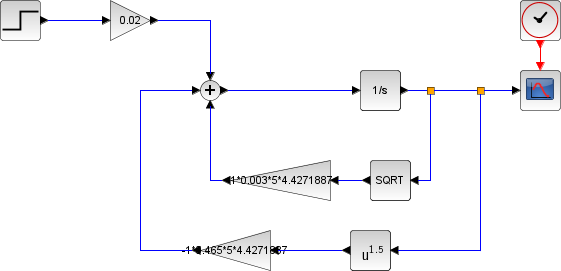
\includegraphics[scale=0.8]{scheme4}
	\caption{Структурная схема моделирования флотационной машины}
	\label{p:Флотационная_машина_схема}
\end{figure}


\begin{figure}[h!]
	\centering
	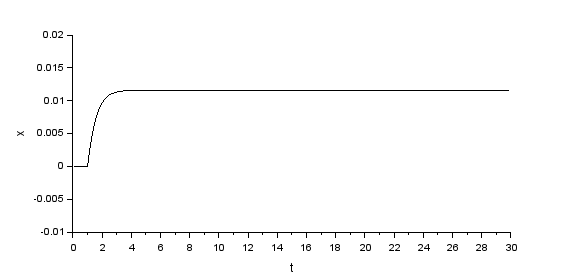
\includegraphics[scale=0.8]{graph4-1}
	\caption{Графики изменения уровня жидкости/пульпы в флотационной машине }
	\label{p:Флотационная_машина_графики}
\end{figure}

\end{document}
